\documentclass{article}
\usepackage[utf8]{inputenc} %кодировка
\usepackage[T2A]{fontenc}
\usepackage[english,russian]{babel} %русификатор 
\usepackage{mathtools} %библиотека матеши
\usepackage[left=1cm,right=1cm,top=2cm,bottom=2cm,bindingoffset=0cm]{geometry} %изменение отступов на листе
\usepackage{amsmath}
\usepackage{graphicx} %библиотека для графики и картинок
\graphicspath{}
\DeclareGraphicsExtensions{.pdf,.png,.jpg}
\usepackage{subcaption}
\usepackage{pgfplots}
\usepackage{float}

\begin{document}

\section{SB p 71 ex5  }
(напишите свои идеи, используйте Second Conditional)

1. I would be terrified to death if I saw a mouse in my kitchen

2. I would try to scare the dog if I saw a dog attacking someone

3. I would be anxious if a bird or a bat flew into my bedroom

4. I would start looking for a new home on another planet if I saw a large spider in the bath

5. I would go towards the McDonald's if it was a very hot day and I were on a beach that was famous for shark attacks

6. I would feel panic if someone offered to buy my a fur coat

7. I would feel dizzy all next day if my neighbour's dog barked all night

8. If a friend asked me to look after their cat or dog for the weekend, I wouldn't agree, because I sleep on the weekend

9. If I went to somebody's house for dinner and they gave you kangaroo, I would be nauseous
\section{SB p 73 ex5}
(напишите ответы для вас, используйте Present Perfect)

1. I have had a small Corgi dog since last year.

2. I have had a large note-taking tablet for three years.

3.  have lived in a modern dorm for two years.

4. I have lived near this school for two years. It's five hundred meters from me.

5. I have a friend from Germany and I know he has been living there since he was eighteen.

6. I have been a fan of the local football team ever since I was a child.

7. I have been a member of the sports club for about two years.

8. I haven't been married for nineteen years, so my partner doesn't have a name because he doesn't come for nineteen years.
\end{document}
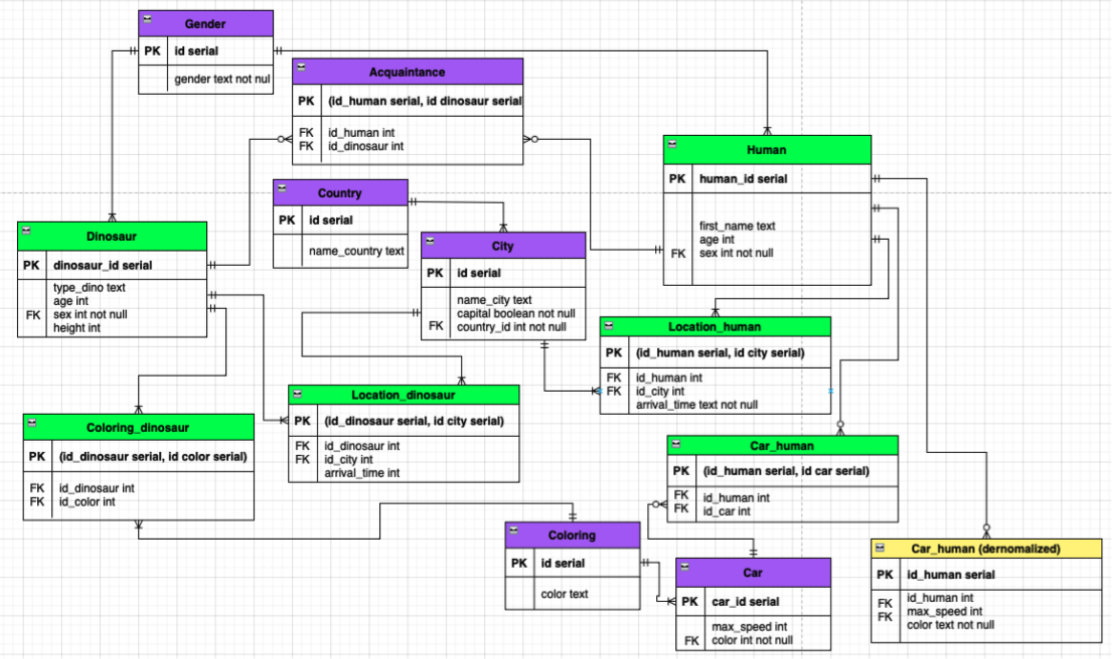
\includegraphics[width=.9\textwidth]{123}